\documentclass{article}
\usepackage{graphicx}
\begin{document}
	\section*{Lsg Vorschlag ADSÜ11 A1 Maximilian Maag}
	\subsection*{Aufgabe 1}
	Der illustrierte Baum entsteht durch das Einfügen von 11, 17, 29, 15, 3, 7, 31, 19, 23.
	Der Vorgang ist nachstehend beispielhaft dargestellt. \\ \\
	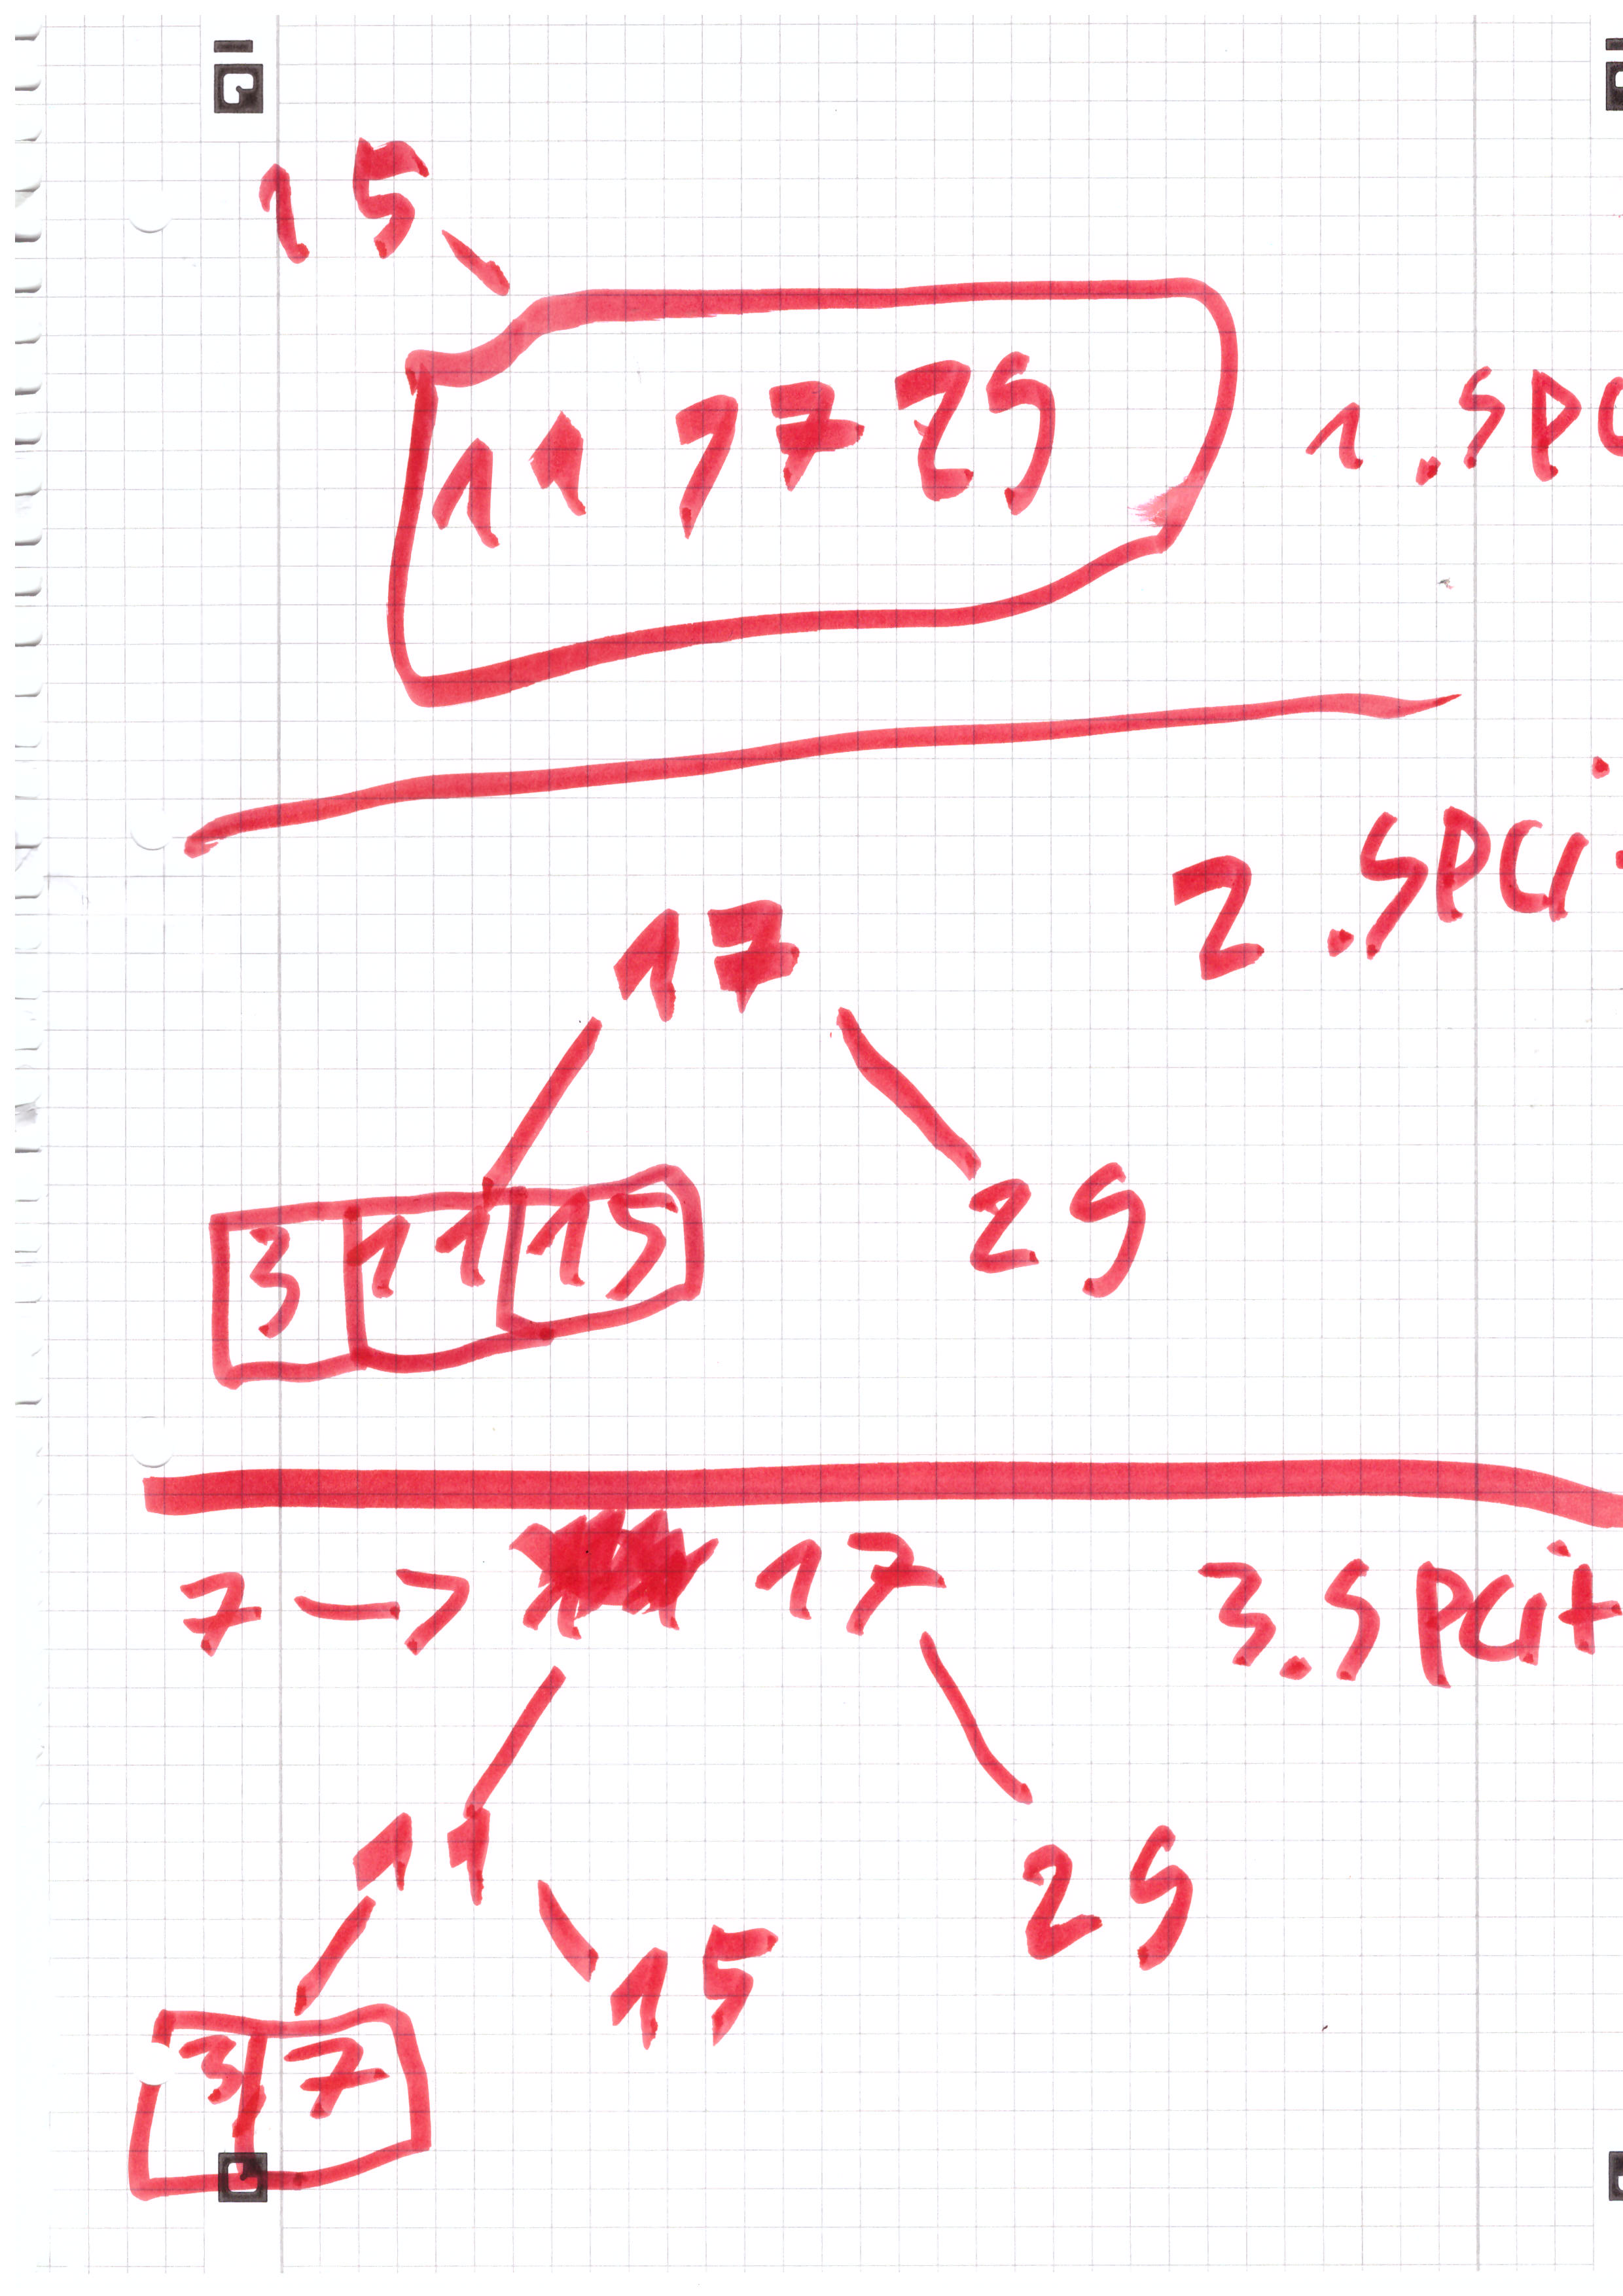
\includegraphics[width=\linewidth]{A10101} \\
	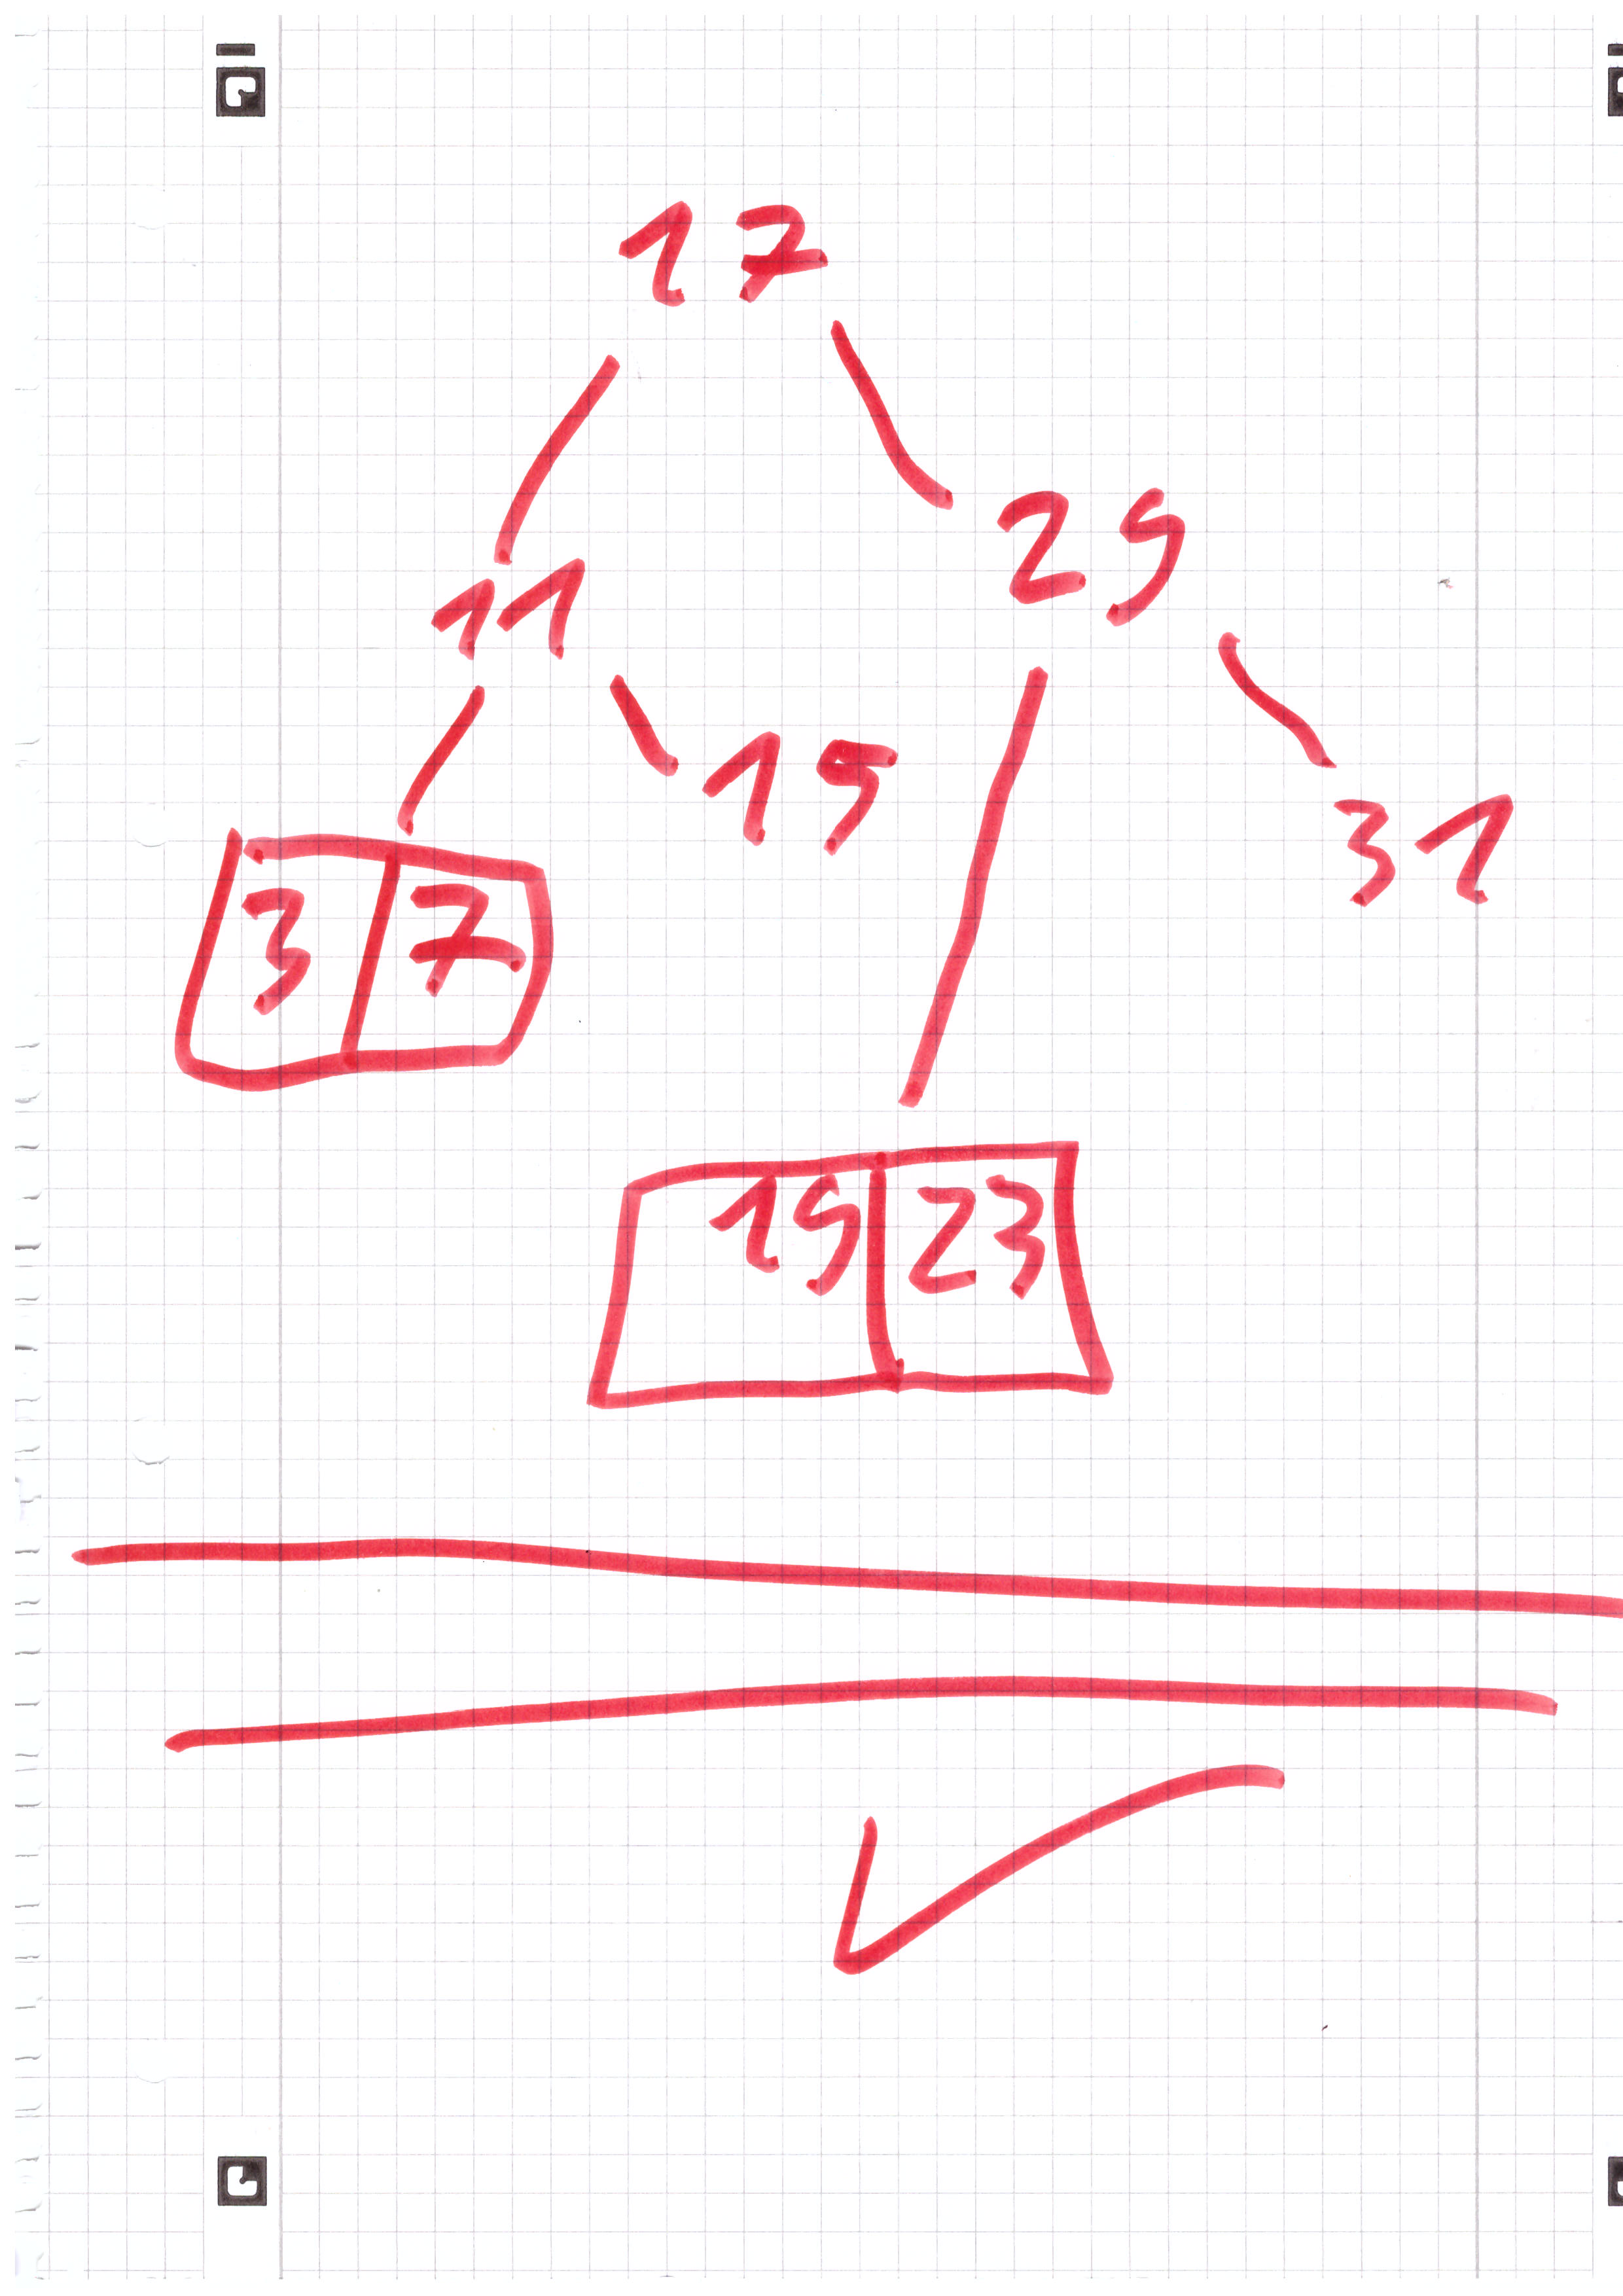
\includegraphics[width=\linewidth]{A10102}
	\subsection*{Aufgabe 2}
	Durch eine andere Reihenfolge lässt sich ein anderer Baum illustrieren. \\
	\\
	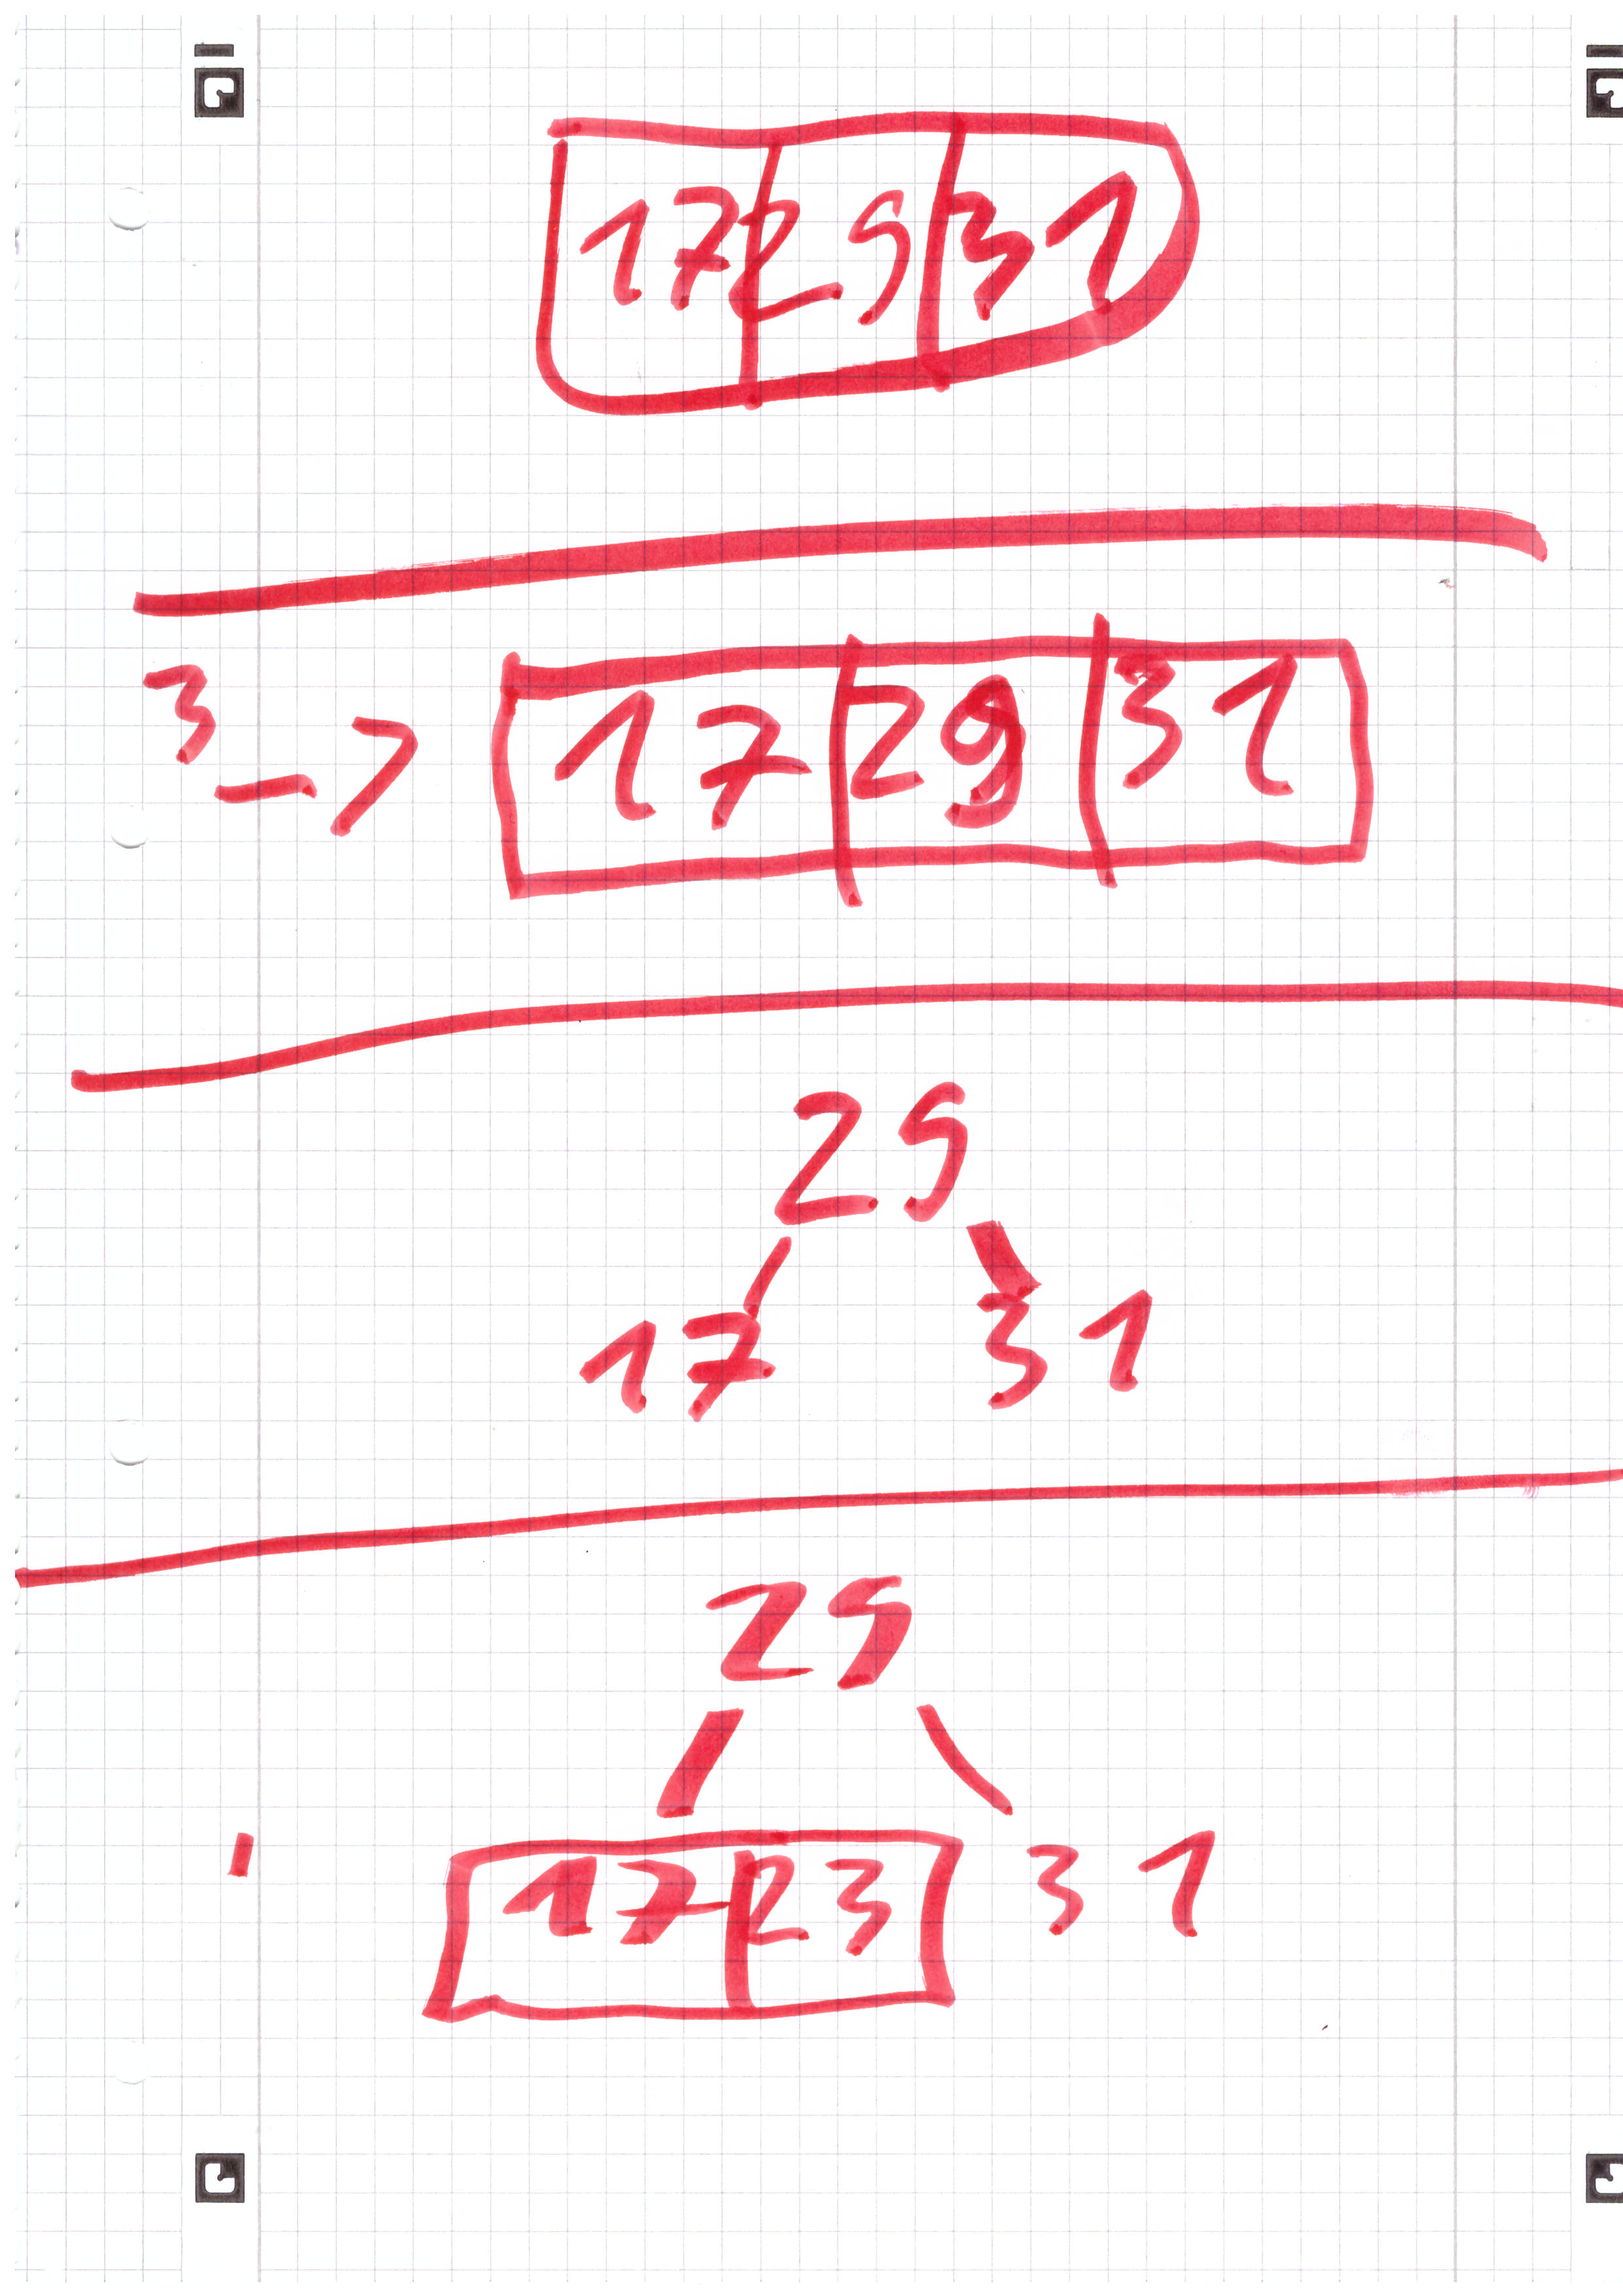
\includegraphics[width=\linewidth]{A10201} \\ \\
	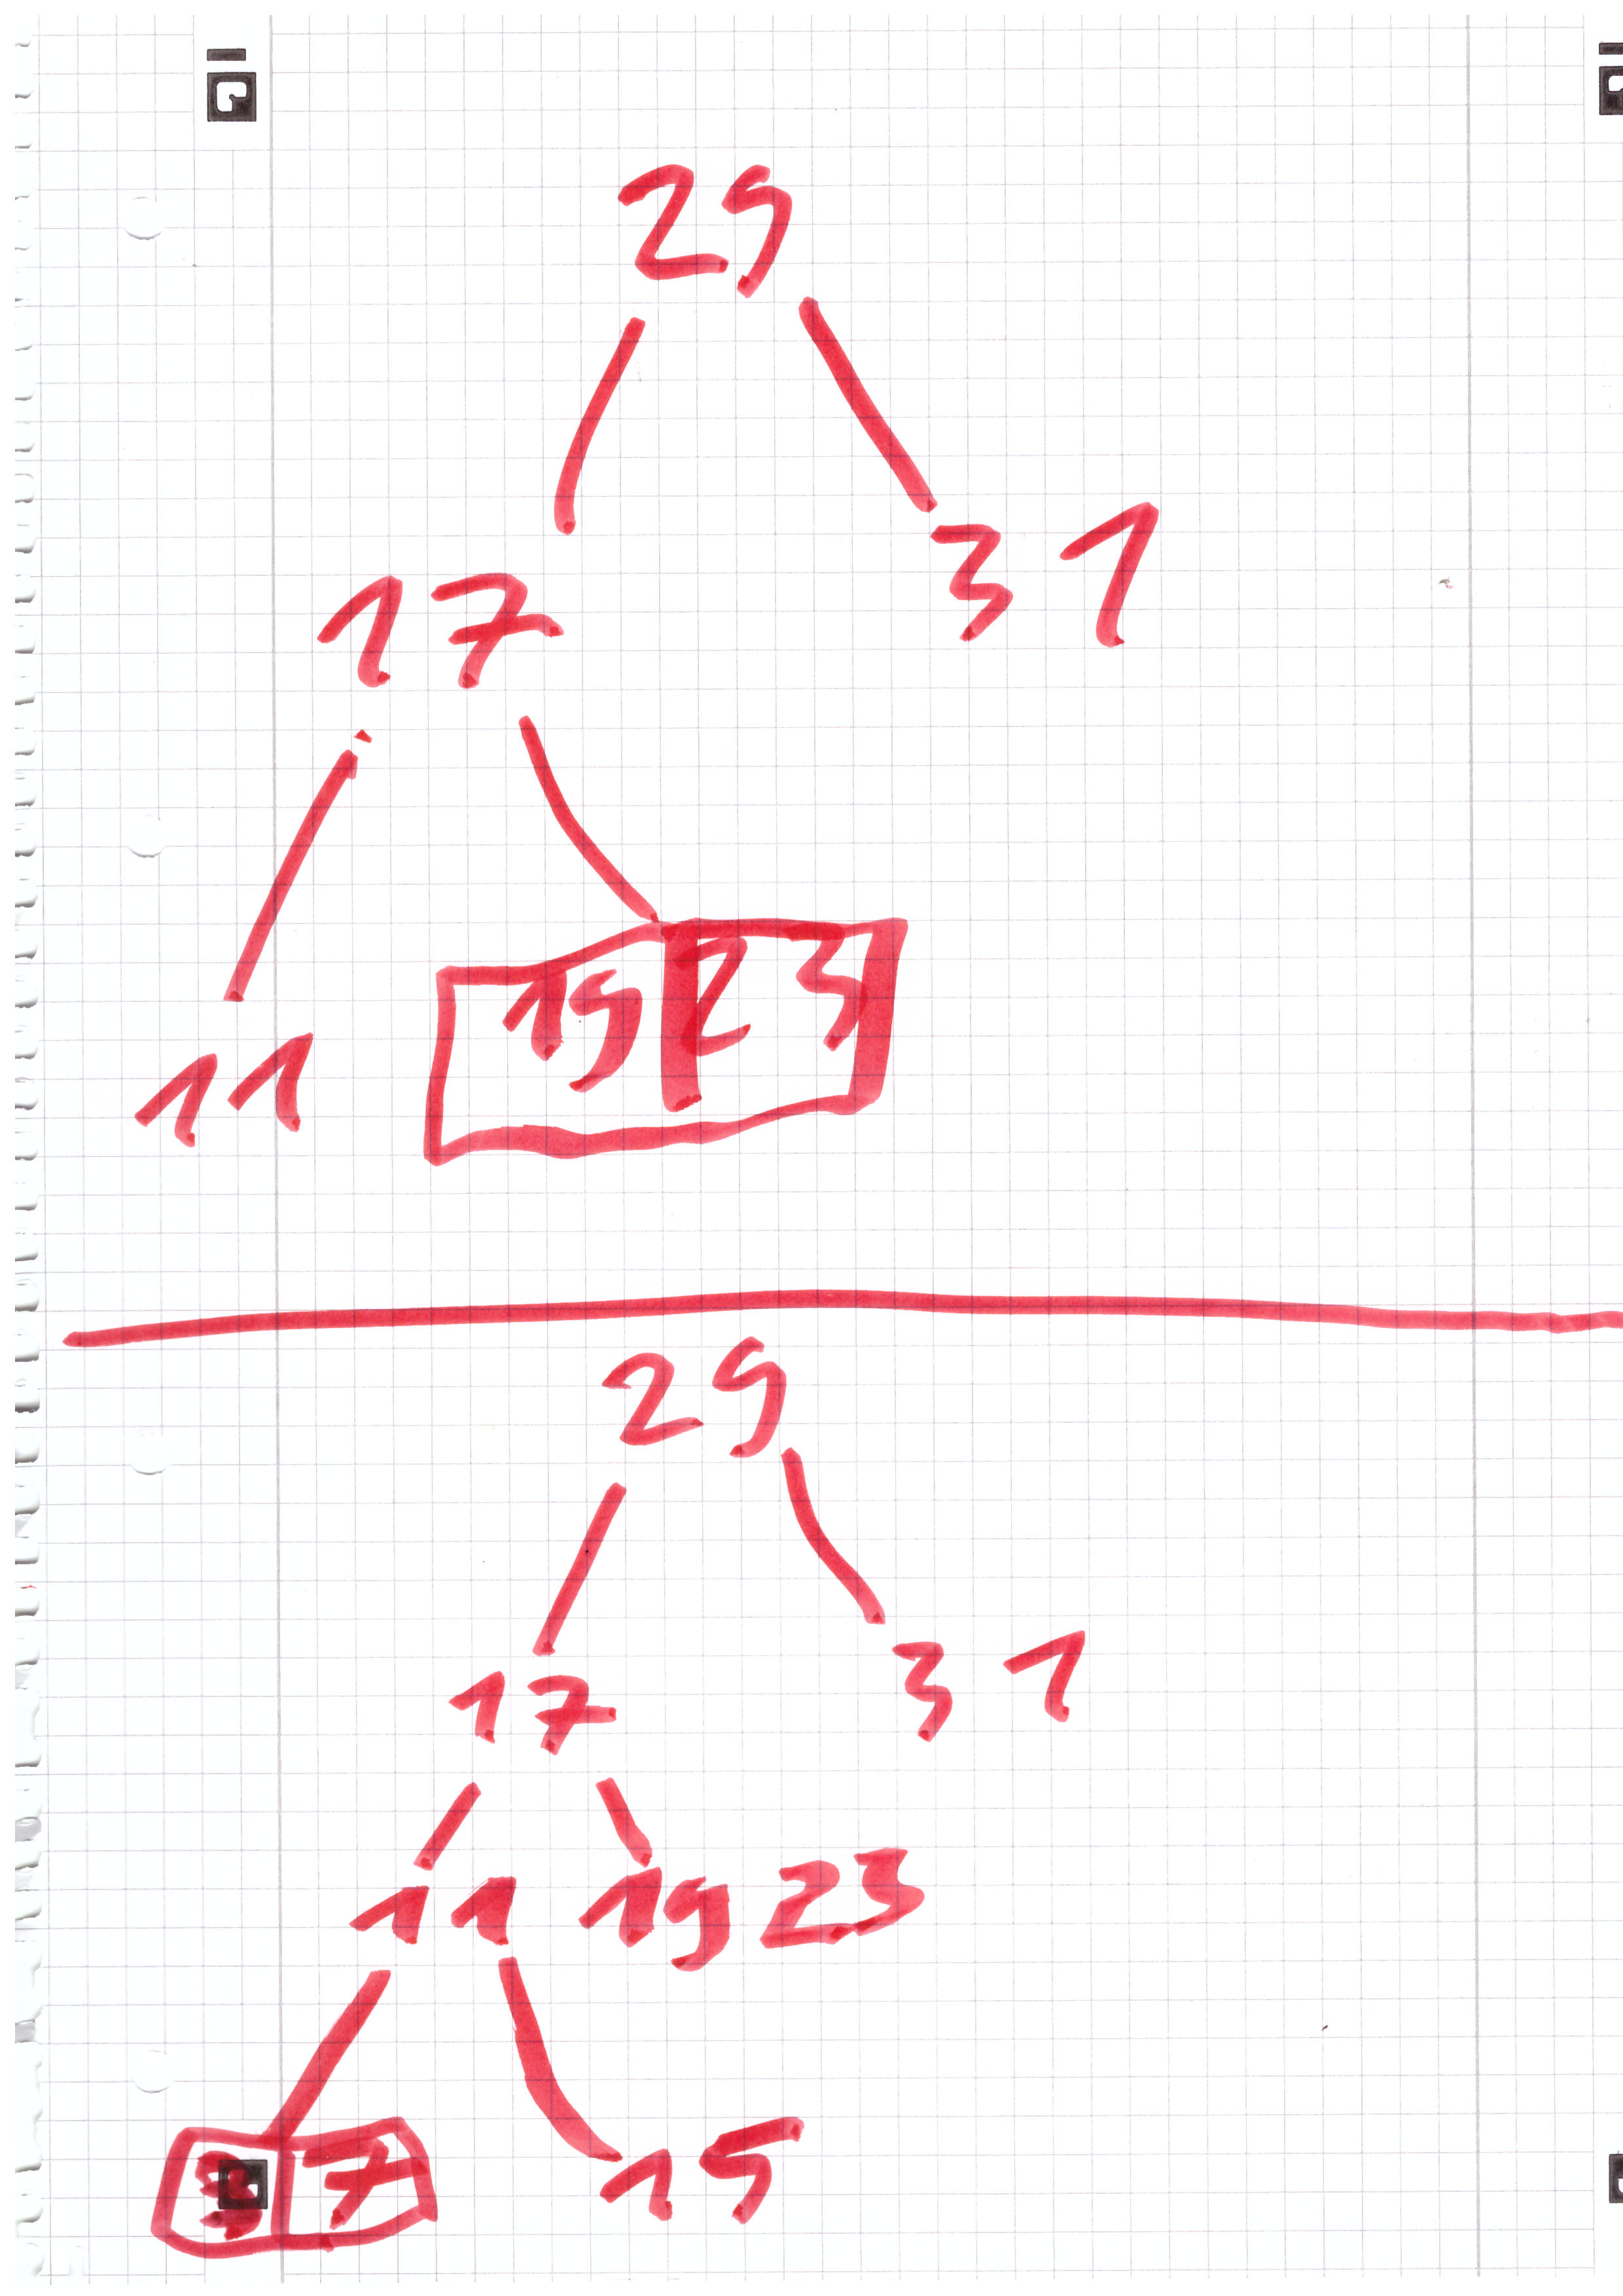
\includegraphics[width=\linewidth]{A10202}
\end{document}